% Options for packages loaded elsewhere
\PassOptionsToPackage{unicode}{hyperref}
\PassOptionsToPackage{hyphens}{url}
%
\documentclass[
]{article}
\usepackage{amsmath,amssymb}
\usepackage{lmodern}
\usepackage{ifxetex,ifluatex}
\ifnum 0\ifxetex 1\fi\ifluatex 1\fi=0 % if pdftex
  \usepackage[T1]{fontenc}
  \usepackage[utf8]{inputenc}
  \usepackage{textcomp} % provide euro and other symbols
\else % if luatex or xetex
  \usepackage{unicode-math}
  \defaultfontfeatures{Scale=MatchLowercase}
  \defaultfontfeatures[\rmfamily]{Ligatures=TeX,Scale=1}
\fi
% Use upquote if available, for straight quotes in verbatim environments
\IfFileExists{upquote.sty}{\usepackage{upquote}}{}
\IfFileExists{microtype.sty}{% use microtype if available
  \usepackage[]{microtype}
  \UseMicrotypeSet[protrusion]{basicmath} % disable protrusion for tt fonts
}{}
\makeatletter
\@ifundefined{KOMAClassName}{% if non-KOMA class
  \IfFileExists{parskip.sty}{%
    \usepackage{parskip}
  }{% else
    \setlength{\parindent}{0pt}
    \setlength{\parskip}{6pt plus 2pt minus 1pt}}
}{% if KOMA class
  \KOMAoptions{parskip=half}}
\makeatother
\usepackage{xcolor}
\IfFileExists{xurl.sty}{\usepackage{xurl}}{} % add URL line breaks if available
\IfFileExists{bookmark.sty}{\usepackage{bookmark}}{\usepackage{hyperref}}
\hypersetup{
  hidelinks,
  pdfcreator={LaTeX via pandoc}}
\urlstyle{same} % disable monospaced font for URLs
\usepackage[margin=1in]{geometry}
\usepackage{color}
\usepackage{fancyvrb}
\newcommand{\VerbBar}{|}
\newcommand{\VERB}{\Verb[commandchars=\\\{\}]}
\DefineVerbatimEnvironment{Highlighting}{Verbatim}{commandchars=\\\{\}}
% Add ',fontsize=\small' for more characters per line
\usepackage{framed}
\definecolor{shadecolor}{RGB}{248,248,248}
\newenvironment{Shaded}{\begin{snugshade}}{\end{snugshade}}
\newcommand{\AlertTok}[1]{\textcolor[rgb]{0.94,0.16,0.16}{#1}}
\newcommand{\AnnotationTok}[1]{\textcolor[rgb]{0.56,0.35,0.01}{\textbf{\textit{#1}}}}
\newcommand{\AttributeTok}[1]{\textcolor[rgb]{0.77,0.63,0.00}{#1}}
\newcommand{\BaseNTok}[1]{\textcolor[rgb]{0.00,0.00,0.81}{#1}}
\newcommand{\BuiltInTok}[1]{#1}
\newcommand{\CharTok}[1]{\textcolor[rgb]{0.31,0.60,0.02}{#1}}
\newcommand{\CommentTok}[1]{\textcolor[rgb]{0.56,0.35,0.01}{\textit{#1}}}
\newcommand{\CommentVarTok}[1]{\textcolor[rgb]{0.56,0.35,0.01}{\textbf{\textit{#1}}}}
\newcommand{\ConstantTok}[1]{\textcolor[rgb]{0.00,0.00,0.00}{#1}}
\newcommand{\ControlFlowTok}[1]{\textcolor[rgb]{0.13,0.29,0.53}{\textbf{#1}}}
\newcommand{\DataTypeTok}[1]{\textcolor[rgb]{0.13,0.29,0.53}{#1}}
\newcommand{\DecValTok}[1]{\textcolor[rgb]{0.00,0.00,0.81}{#1}}
\newcommand{\DocumentationTok}[1]{\textcolor[rgb]{0.56,0.35,0.01}{\textbf{\textit{#1}}}}
\newcommand{\ErrorTok}[1]{\textcolor[rgb]{0.64,0.00,0.00}{\textbf{#1}}}
\newcommand{\ExtensionTok}[1]{#1}
\newcommand{\FloatTok}[1]{\textcolor[rgb]{0.00,0.00,0.81}{#1}}
\newcommand{\FunctionTok}[1]{\textcolor[rgb]{0.00,0.00,0.00}{#1}}
\newcommand{\ImportTok}[1]{#1}
\newcommand{\InformationTok}[1]{\textcolor[rgb]{0.56,0.35,0.01}{\textbf{\textit{#1}}}}
\newcommand{\KeywordTok}[1]{\textcolor[rgb]{0.13,0.29,0.53}{\textbf{#1}}}
\newcommand{\NormalTok}[1]{#1}
\newcommand{\OperatorTok}[1]{\textcolor[rgb]{0.81,0.36,0.00}{\textbf{#1}}}
\newcommand{\OtherTok}[1]{\textcolor[rgb]{0.56,0.35,0.01}{#1}}
\newcommand{\PreprocessorTok}[1]{\textcolor[rgb]{0.56,0.35,0.01}{\textit{#1}}}
\newcommand{\RegionMarkerTok}[1]{#1}
\newcommand{\SpecialCharTok}[1]{\textcolor[rgb]{0.00,0.00,0.00}{#1}}
\newcommand{\SpecialStringTok}[1]{\textcolor[rgb]{0.31,0.60,0.02}{#1}}
\newcommand{\StringTok}[1]{\textcolor[rgb]{0.31,0.60,0.02}{#1}}
\newcommand{\VariableTok}[1]{\textcolor[rgb]{0.00,0.00,0.00}{#1}}
\newcommand{\VerbatimStringTok}[1]{\textcolor[rgb]{0.31,0.60,0.02}{#1}}
\newcommand{\WarningTok}[1]{\textcolor[rgb]{0.56,0.35,0.01}{\textbf{\textit{#1}}}}
\usepackage{graphicx}
\makeatletter
\def\maxwidth{\ifdim\Gin@nat@width>\linewidth\linewidth\else\Gin@nat@width\fi}
\def\maxheight{\ifdim\Gin@nat@height>\textheight\textheight\else\Gin@nat@height\fi}
\makeatother
% Scale images if necessary, so that they will not overflow the page
% margins by default, and it is still possible to overwrite the defaults
% using explicit options in \includegraphics[width, height, ...]{}
\setkeys{Gin}{width=\maxwidth,height=\maxheight,keepaspectratio}
% Set default figure placement to htbp
\makeatletter
\def\fps@figure{htbp}
\makeatother
\setlength{\emergencystretch}{3em} % prevent overfull lines
\providecommand{\tightlist}{%
  \setlength{\itemsep}{0pt}\setlength{\parskip}{0pt}}
\setcounter{secnumdepth}{-\maxdimen} % remove section numbering
\ifluatex
  \usepackage{selnolig}  % disable illegal ligatures
\fi

\author{}
\date{\vspace{-2.5em}}

\begin{document}

Clear workspace and load libraries

\begin{Shaded}
\begin{Highlighting}[]
\FunctionTok{rm}\NormalTok{(}\AttributeTok{list =} \FunctionTok{ls}\NormalTok{())}
\CommentTok{\# Load libraries}
\FunctionTok{library}\NormalTok{(tidyverse)}
\end{Highlighting}
\end{Shaded}

\begin{verbatim}
## -- Attaching packages --------------------------------------- tidyverse 1.3.1 --
\end{verbatim}

\begin{verbatim}
## v ggplot2 3.3.5     v purrr   0.3.4
## v tibble  3.1.6     v dplyr   1.0.7
## v tidyr   1.1.4     v stringr 1.4.0
## v readr   2.1.0     v forcats 0.5.1
\end{verbatim}

\begin{verbatim}
## Warning: package 'tibble' was built under R version 4.1.2
\end{verbatim}

\begin{verbatim}
## Warning: package 'readr' was built under R version 4.1.2
\end{verbatim}

\begin{verbatim}
## -- Conflicts ------------------------------------------ tidyverse_conflicts() --
## x dplyr::filter() masks stats::filter()
## x dplyr::lag()    masks stats::lag()
\end{verbatim}

\begin{Shaded}
\begin{Highlighting}[]
\FunctionTok{library}\NormalTok{(MASS)}
\end{Highlighting}
\end{Shaded}

\begin{verbatim}
## Warning: package 'MASS' was built under R version 4.1.2
\end{verbatim}

\begin{verbatim}
## 
## Attaching package: 'MASS'
\end{verbatim}

\begin{verbatim}
## The following object is masked from 'package:dplyr':
## 
##     select
\end{verbatim}

\begin{Shaded}
\begin{Highlighting}[]
\FunctionTok{library}\NormalTok{(psych)}
\end{Highlighting}
\end{Shaded}

\begin{verbatim}
## 
## Attaching package: 'psych'
\end{verbatim}

\begin{verbatim}
## The following objects are masked from 'package:ggplot2':
## 
##     %+%, alpha
\end{verbatim}

\begin{Shaded}
\begin{Highlighting}[]
\FunctionTok{library}\NormalTok{(ggbiplot)}
\end{Highlighting}
\end{Shaded}

\begin{verbatim}
## Loading required package: plyr
\end{verbatim}

\begin{verbatim}
## ------------------------------------------------------------------------------
\end{verbatim}

\begin{verbatim}
## You have loaded plyr after dplyr - this is likely to cause problems.
## If you need functions from both plyr and dplyr, please load plyr first, then dplyr:
## library(plyr); library(dplyr)
\end{verbatim}

\begin{verbatim}
## ------------------------------------------------------------------------------
\end{verbatim}

\begin{verbatim}
## 
## Attaching package: 'plyr'
\end{verbatim}

\begin{verbatim}
## The following objects are masked from 'package:dplyr':
## 
##     arrange, count, desc, failwith, id, mutate, rename, summarise,
##     summarize
\end{verbatim}

\begin{verbatim}
## The following object is masked from 'package:purrr':
## 
##     compact
\end{verbatim}

\begin{verbatim}
## Loading required package: scales
\end{verbatim}

\begin{verbatim}
## 
## Attaching package: 'scales'
\end{verbatim}

\begin{verbatim}
## The following objects are masked from 'package:psych':
## 
##     alpha, rescale
\end{verbatim}

\begin{verbatim}
## The following object is masked from 'package:purrr':
## 
##     discard
\end{verbatim}

\begin{verbatim}
## The following object is masked from 'package:readr':
## 
##     col_factor
\end{verbatim}

\begin{verbatim}
## Loading required package: grid
\end{verbatim}

Data Source:
www.kaggle.com/bryanb/fifa-player-stats-database/version/27?select=FIFA22\_official\_data.csv

How many unique roles/positions are in the dataset?

\begin{Shaded}
\begin{Highlighting}[]
\FunctionTok{length}\NormalTok{(}\FunctionTok{unique}\NormalTok{(raw\_data}\SpecialCharTok{$}\StringTok{\textasciigrave{}}\AttributeTok{Best Position}\StringTok{\textasciigrave{}}\NormalTok{))}
\end{Highlighting}
\end{Shaded}

\begin{verbatim}
## [1] 15
\end{verbatim}

Preprocess the data - we have 15 unique positions - We'd like to make
that number smaller becuase many positions are very similar - We can
divide them into following categories: - Center Forward - Center
Midfielder - Right Midfielder/Winger - Left Midfielder/Winger - Right
Back - Left Back - Central Back (defender) - Goalkeeper

\begin{Shaded}
\begin{Highlighting}[]
\NormalTok{data }\OtherTok{\textless{}{-}}\NormalTok{ raw\_data }\SpecialCharTok{\%\textgreater{}\%}
    \CommentTok{\# Reduction of positions}
\NormalTok{    dplyr}\SpecialCharTok{::}\FunctionTok{mutate}\NormalTok{(}
        \AttributeTok{BestPos =} \FunctionTok{factor}\NormalTok{(}
            \FunctionTok{case\_when}\NormalTok{(}
                \StringTok{\textasciigrave{}}\AttributeTok{Best Position}\StringTok{\textasciigrave{}} \SpecialCharTok{\%in\%} \FunctionTok{c}\NormalTok{(}\StringTok{"CF"}\NormalTok{, }\StringTok{"ST"}\NormalTok{) }\SpecialCharTok{\textasciitilde{}} \StringTok{"CF/ST"}\NormalTok{,}
                \StringTok{\textasciigrave{}}\AttributeTok{Best Position}\StringTok{\textasciigrave{}}  \SpecialCharTok{\%in\%} \FunctionTok{c}\NormalTok{(}\StringTok{"CAM"}\NormalTok{, }\StringTok{"CM"}\NormalTok{, }\StringTok{"CDM"}\NormalTok{) }\SpecialCharTok{\textasciitilde{}} \StringTok{"CM/CAM/CDM"}\NormalTok{,}
                \StringTok{\textasciigrave{}}\AttributeTok{Best Position}\StringTok{\textasciigrave{}} \SpecialCharTok{\%in\%} \FunctionTok{c}\NormalTok{(}\StringTok{"RW"}\NormalTok{, }\StringTok{"RM"}\NormalTok{) }\SpecialCharTok{\textasciitilde{}} \StringTok{"RW/RM"}\NormalTok{,}
                \StringTok{\textasciigrave{}}\AttributeTok{Best Position}\StringTok{\textasciigrave{}} \SpecialCharTok{\%in\%} \FunctionTok{c}\NormalTok{(}\StringTok{"LW"}\NormalTok{, }\StringTok{"LM"}\NormalTok{) }\SpecialCharTok{\textasciitilde{}} \StringTok{"LW/RM"}\NormalTok{,}
                \StringTok{\textasciigrave{}}\AttributeTok{Best Position}\StringTok{\textasciigrave{}} \SpecialCharTok{\%in\%} \FunctionTok{c}\NormalTok{(}\StringTok{"RWB"}\NormalTok{, }\StringTok{"RB"}\NormalTok{) }\SpecialCharTok{\textasciitilde{}} \StringTok{"RWB/RB"}\NormalTok{,}
                \StringTok{\textasciigrave{}}\AttributeTok{Best Position}\StringTok{\textasciigrave{}} \SpecialCharTok{\%in\%} \FunctionTok{c}\NormalTok{(}\StringTok{"LWB"}\NormalTok{, }\StringTok{"LB"}\NormalTok{) }\SpecialCharTok{\textasciitilde{}} \StringTok{"LWB/LB"}\NormalTok{,}
                \StringTok{\textasciigrave{}}\AttributeTok{Best Position}\StringTok{\textasciigrave{}} \SpecialCharTok{\%in\%} \FunctionTok{c}\NormalTok{(}\StringTok{"CB"}\NormalTok{) }\SpecialCharTok{\textasciitilde{}} \StringTok{"CB"}\NormalTok{,}
                \StringTok{\textasciigrave{}}\AttributeTok{Best Position}\StringTok{\textasciigrave{}} \SpecialCharTok{\%in\%} \FunctionTok{c}\NormalTok{(}\StringTok{"GK"}\NormalTok{) }\SpecialCharTok{\textasciitilde{}} \StringTok{"GK"}
\NormalTok{            )}
\NormalTok{        ),}
        \AttributeTok{Height =} \FunctionTok{as.double}\NormalTok{(}\FunctionTok{str\_replace}\NormalTok{(Height, }\StringTok{\textquotesingle{}cm\textquotesingle{}}\NormalTok{, }\StringTok{\textquotesingle{}\textquotesingle{}}\NormalTok{)),}
        \AttributeTok{Weight =} \FunctionTok{as.double}\NormalTok{(}\FunctionTok{str\_replace}\NormalTok{(Weight, }\StringTok{\textquotesingle{}kg\textquotesingle{}}\NormalTok{, }\StringTok{\textquotesingle{}\textquotesingle{}}\NormalTok{)),}
        \AttributeTok{PrefFoot =} \FunctionTok{as.factor}\NormalTok{(}\StringTok{\textasciigrave{}}\AttributeTok{Preferred Foot}\StringTok{\textasciigrave{}}\NormalTok{),}
        \AttributeTok{WeekFoot =} \StringTok{\textasciigrave{}}\AttributeTok{Weak Foot}\StringTok{\textasciigrave{}}\NormalTok{,}
        \AttributeTok{SkillMoves =} \StringTok{\textasciigrave{}}\AttributeTok{Skill Moves}\StringTok{\textasciigrave{}}\NormalTok{,}
        \AttributeTok{WorkRate =} \FunctionTok{as.factor}\NormalTok{(}\StringTok{\textasciigrave{}}\AttributeTok{Work Rate}\StringTok{\textasciigrave{}}\NormalTok{),}
        \AttributeTok{BodyType =} \FunctionTok{factor}\NormalTok{(}\StringTok{\textasciigrave{}}\AttributeTok{Body Type}\StringTok{\textasciigrave{}}\NormalTok{)}
\NormalTok{    ) }\SpecialCharTok{\%\textgreater{}\%}
    \CommentTok{\# Picking only relevant columns}
\NormalTok{    dplyr}\SpecialCharTok{::}\FunctionTok{select}\NormalTok{(}
\NormalTok{        Name,}
\NormalTok{        BestPos,}
\NormalTok{        Age,}
\NormalTok{        PrefFoot,}
\NormalTok{        WeekFoot,}
\NormalTok{        SkillMoves,}
\NormalTok{        WorkRate,}
\NormalTok{        BodyType,}
\NormalTok{        Height,}
\NormalTok{        Weight,}
\NormalTok{        Crossing,}
\NormalTok{        Finishing,}
\NormalTok{        HeadingAccuracy,}
\NormalTok{        ShortPassing,}
\NormalTok{        Volleys,}
\NormalTok{        Dribbling,}
\NormalTok{        Curve,}
\NormalTok{        FKAccuracy,}
\NormalTok{        LongPassing,}
\NormalTok{        BallControl,}
\NormalTok{        Acceleration,}
\NormalTok{        SprintSpeed,}
\NormalTok{        Agility,}
\NormalTok{        Reactions,}
\NormalTok{        Stamina,}
\NormalTok{        Interceptions,}
\NormalTok{        Balance,}
\NormalTok{        Strength,}
\NormalTok{        Positioning,}
\NormalTok{        ShotPower,}
\NormalTok{        LongShots,}
\NormalTok{        Vision,}
\NormalTok{        StandingTackle,}
\NormalTok{        Jumping,}
\NormalTok{        Aggression,}
\NormalTok{        Penalties,}
\NormalTok{        SlidingTackle}
\NormalTok{    ) }
\end{Highlighting}
\end{Shaded}

\begin{itemize}
\tightlist
\item
  To make the prediction even simpler, we will predict only Centre
  Forwards and Central Midfielders - These two categories should be
  quite different and we expect LDA to perform well
\item
  To make the prediction simpler, we use only numeric variables, thus we
  exclude categorical columns
\end{itemize}

\begin{Shaded}
\begin{Highlighting}[]
\NormalTok{fifa }\OtherTok{\textless{}{-}}\NormalTok{ data }\SpecialCharTok{\%\textgreater{}\%}
    \FunctionTok{filter}\NormalTok{(BestPos }\SpecialCharTok{\%in\%} \FunctionTok{c}\NormalTok{(}\StringTok{"CM/CAM/CDM"}\NormalTok{, }\StringTok{"CF/ST"}\NormalTok{)) }\SpecialCharTok{\%\textgreater{}\%}
    \CommentTok{\# Ponechame si vsak iba numericke stlpce}
    \FunctionTok{select\_if}\NormalTok{(}\SpecialCharTok{!}\NormalTok{(}\FunctionTok{map}\NormalTok{(., class) }\SpecialCharTok{\%in\%} \FunctionTok{c}\NormalTok{(}\StringTok{"factor"}\NormalTok{, }\StringTok{"character"}\NormalTok{)))}
\end{Highlighting}
\end{Shaded}

\begin{Shaded}
\begin{Highlighting}[]
\CommentTok{\# Number of NA values}
\FunctionTok{str\_glue}\NormalTok{(}\StringTok{\textquotesingle{}\{round(sum(is.na(fifa)) / dim(fifa)[1] * 100, 2)\} \%\textquotesingle{}}\NormalTok{)}
\end{Highlighting}
\end{Shaded}

\begin{verbatim}
## 2.93 %
\end{verbatim}

Only 3\% of rows contain missing values - we can drop those

\begin{Shaded}
\begin{Highlighting}[]
\NormalTok{fifa }\OtherTok{\textless{}{-}}\NormalTok{ fifa }\SpecialCharTok{\%\textgreater{}\%}
    \FunctionTok{na.omit}\NormalTok{()}
\CommentTok{\# Contorl check of missing values}
\FunctionTok{sum}\NormalTok{(}\FunctionTok{is.na}\NormalTok{(fifa))}
\end{Highlighting}
\end{Shaded}

\begin{verbatim}
## [1] 0
\end{verbatim}

In next step, we perform PCA to see whether it can, keep substantional
amount of variance in first three Principal Components. The number 3
comes from the knowledge of the columns. They could be roughly divided
into 3 categories: Offensive, Defensive and Physical attributes

\begin{Shaded}
\begin{Highlighting}[]
\CommentTok{\# Fit PCA on standardized and centered data}
\NormalTok{fit }\OtherTok{\textless{}{-}} \FunctionTok{prcomp}\NormalTok{(fifa, }\AttributeTok{center =}\NormalTok{ T, }\AttributeTok{scale. =}\NormalTok{ T)}
\CommentTok{\# Show results}
\NormalTok{sum\_pca }\OtherTok{\textless{}{-}} \FunctionTok{summary}\NormalTok{(fit) }
\NormalTok{sum\_pca}
\end{Highlighting}
\end{Shaded}

\begin{verbatim}
## Importance of components:
##                           PC1    PC2    PC3     PC4     PC5     PC6     PC7
## Standard deviation     3.2114 2.3791 2.1818 1.49468 1.09013 0.94982 0.85284
## Proportion of Variance 0.3223 0.1769 0.1488 0.06982 0.03714 0.02819 0.02273
## Cumulative Proportion  0.3223 0.4992 0.6479 0.71773 0.75487 0.78306 0.80579
##                            PC8     PC9    PC10    PC11    PC12    PC13    PC14
## Standard deviation     0.77856 0.72361 0.69902 0.64652 0.63006 0.58375 0.57218
## Proportion of Variance 0.01894 0.01636 0.01527 0.01306 0.01241 0.01065 0.01023
## Cumulative Proportion  0.82474 0.84110 0.85637 0.86943 0.88184 0.89248 0.90272
##                           PC15    PC16    PC17    PC18    PC19    PC20    PC21
## Standard deviation     0.54945 0.53306 0.51456 0.49619 0.47960 0.45674 0.45173
## Proportion of Variance 0.00943 0.00888 0.00827 0.00769 0.00719 0.00652 0.00638
## Cumulative Proportion  0.91215 0.92103 0.92930 0.93700 0.94419 0.95070 0.95708
##                           PC22    PC23    PC24    PC25   PC26    PC27    PC28
## Standard deviation     0.43188 0.42434 0.42088 0.40959 0.3754 0.34597 0.33975
## Proportion of Variance 0.00583 0.00563 0.00554 0.00524 0.0044 0.00374 0.00361
## Cumulative Proportion  0.96291 0.96854 0.97407 0.97932 0.9837 0.98746 0.99107
##                           PC29    PC30    PC31    PC32
## Standard deviation     0.30633 0.28678 0.27509 0.18461
## Proportion of Variance 0.00293 0.00257 0.00236 0.00107
## Cumulative Proportion  0.99400 0.99657 0.99893 1.00000
\end{verbatim}

If we were to reduce the dimensionality, we would be probably satisfied
with 75\% variance retained (5 PCs). But let's make a Scree Plot

\begin{Shaded}
\begin{Highlighting}[]
\NormalTok{cum\_var\_pca }\OtherTok{\textless{}{-}}
    \FunctionTok{as.vector}\NormalTok{(}\FunctionTok{sort}\NormalTok{(sum\_pca}\SpecialCharTok{$}\NormalTok{importance[}\DecValTok{2}\NormalTok{, }\DecValTok{1}\SpecialCharTok{:}\DecValTok{10}\NormalTok{], }\AttributeTok{decreasing =} \ConstantTok{TRUE}\NormalTok{))}
\FunctionTok{plot}\NormalTok{(cum\_var\_pca, }\AttributeTok{type =} \StringTok{"l"}\NormalTok{, }
     \AttributeTok{xlab =} \StringTok{"Principal Components"}\NormalTok{, }\AttributeTok{ylab =} \StringTok{"Proportion of Variance"}\NormalTok{,)}
\FunctionTok{axis}\NormalTok{(}\DecValTok{1}\NormalTok{, }\AttributeTok{at=}\FunctionTok{seq}\NormalTok{(}\DecValTok{1}\NormalTok{, }\DecValTok{10}\NormalTok{), }\AttributeTok{labels =} \FunctionTok{as.character}\NormalTok{(}\FunctionTok{seq}\NormalTok{(}\DecValTok{1}\NormalTok{, }\DecValTok{10}\NormalTok{)))}
\FunctionTok{title}\NormalTok{(}\StringTok{"Scree Plot"}\NormalTok{)}
\end{Highlighting}
\end{Shaded}

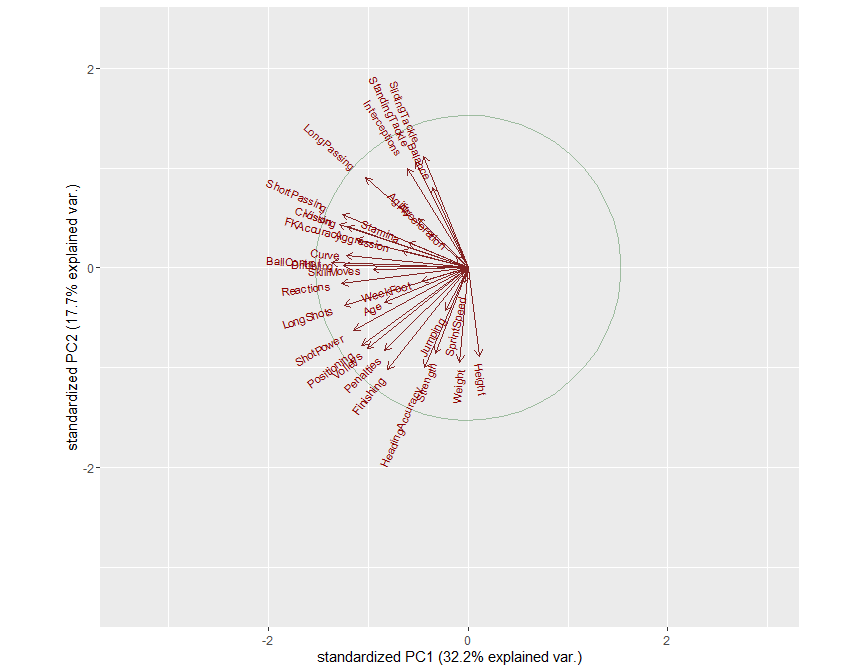
\includegraphics{Kutis_Skuska_markdown_files/figure-latex/unnamed-chunk-9-1.pdf}
Biplot is very helpful in this case

\begin{Shaded}
\begin{Highlighting}[]
\CommentTok{\# Biplot skrz ggplot}
\FunctionTok{ggbiplot}\NormalTok{(}
\NormalTok{    fit,}
    \AttributeTok{scale =} \DecValTok{1}\NormalTok{,}
    \AttributeTok{circle =} \ConstantTok{TRUE}\NormalTok{,}
    \AttributeTok{var.scale =} \DecValTok{1}\NormalTok{,}
    \AttributeTok{var.axes =} \ConstantTok{TRUE}\NormalTok{,}
    \AttributeTok{alpha =} \DecValTok{0}
\NormalTok{)}
\end{Highlighting}
\end{Shaded}

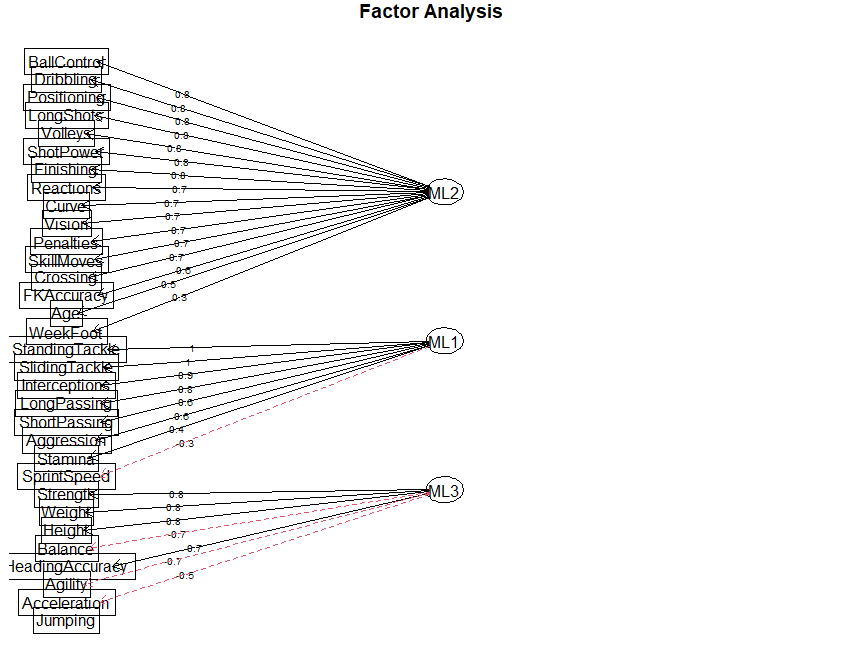
\includegraphics{Kutis_Skuska_markdown_files/figure-latex/unnamed-chunk-10-1.pdf}

Next we perform Factor Analysis. We know approximately how much factors
we should have and we can represent players/positions with smaller
number of columns. Even EA Sports (FIFA 22 producers) summarize the
different players with fewer attributes. They show you their radar plots
in the game. It can be useful to determine which player to play at the
positions, as there are more options usually. We wanna reduce the number
of dimensions only to k=3 because we don't need more and assume no or
only small lost of information. We can see in the diagram that FA
dimension reduction produces what we'd expect. We can name the
dimensions (approximately) as following: - Offensive abilities (ML2) -
Defensive abilities (ML1) - Physical attributes (ML3)

\begin{Shaded}
\begin{Highlighting}[]
\NormalTok{fa }\OtherTok{\textless{}{-}}
    \FunctionTok{fa}\NormalTok{(}
        \AttributeTok{r =}\NormalTok{ fifa,}
        \AttributeTok{nfactors =} \DecValTok{3}\NormalTok{,}
        \AttributeTok{rotate =} \StringTok{"varimax"}\NormalTok{,}
        \AttributeTok{fm =} \StringTok{"ml"}\NormalTok{,}
        \AttributeTok{scores =} \StringTok{"regression"}\NormalTok{,}
        \AttributeTok{residuals =}\NormalTok{ T}
\NormalTok{    )}

\FunctionTok{fa.diagram}\NormalTok{(}\AttributeTok{fa.results =}\NormalTok{ fa)}
\end{Highlighting}
\end{Shaded}

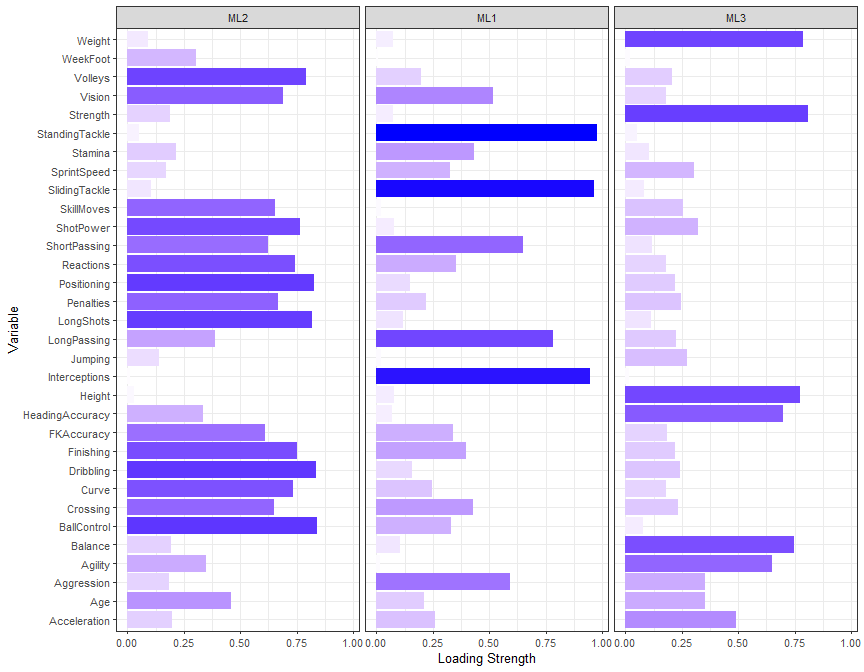
\includegraphics{Kutis_Skuska_markdown_files/figure-latex/unnamed-chunk-11-1.pdf}
In the scatter matrix we can see that the variables are approximately
well divided into 3 clusters. Yes they overlap sometimes, but not
substantionally.

\begin{Shaded}
\begin{Highlighting}[]
\FunctionTok{plot}\NormalTok{(fa)}
\end{Highlighting}
\end{Shaded}

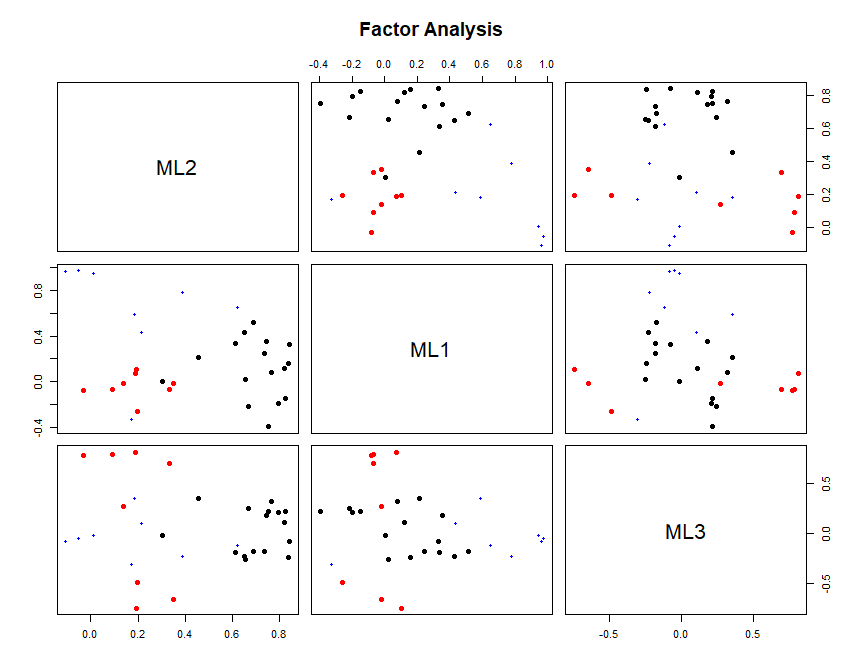
\includegraphics{Kutis_Skuska_markdown_files/figure-latex/unnamed-chunk-12-1.pdf}
In the resulting residual matrix, we see that the non-diagonal values
are close to zero.

\begin{Shaded}
\begin{Highlighting}[]
\NormalTok{fa}\SpecialCharTok{$}\NormalTok{residual}
\end{Highlighting}
\end{Shaded}

\begin{verbatim}
##                          Age      WeekFoot    SkillMoves       Height
## Age              0.622302395  0.0229436174  0.0020785740 -0.142915252
## WeekFoot         0.022943617  0.9077510395  0.0138480711  0.001296898
## SkillMoves       0.002078574  0.0138480711  0.5061073186  0.057989831
## Height          -0.142915252  0.0012968978  0.0579898313  0.392497483
## Weight          -0.036399870  0.0059780405  0.0485009649  0.125347477
## Crossing         0.084850134  0.0060284828  0.0084605236  0.021947715
## Finishing       -0.043146725 -0.0015969419 -0.0197956253 -0.020125170
## HeadingAccuracy -0.003872098 -0.0003851301 -0.0301797934 -0.035166676
## ShortPassing    -0.022805929 -0.0066207039 -0.0136518110  0.026778741
## Volleys          0.064165467  0.0149926991 -0.0058059291 -0.030478818
## Dribbling       -0.117671495 -0.0097555720  0.0655776965  0.066762942
## Curve            0.078352054  0.0202297400  0.0206058241  0.017132893
## FKAccuracy       0.124902099  0.0301307437  0.0091133901 -0.008081374
## LongPassing      0.006581776 -0.0036697434 -0.0108419959  0.032156089
## BallControl     -0.052707780 -0.0042472957  0.0209520426  0.038185459
## Acceleration    -0.213881397 -0.0081180064  0.0276373380  0.023874528
## SprintSpeed     -0.238910901 -0.0132631062  0.0257344001  0.052532028
## Agility         -0.031286142  0.0006404387  0.0332461198 -0.026635413
## Reactions        0.013010434 -0.0155587595 -0.0278754430 -0.035215759
## Stamina         -0.091907427 -0.0027363894 -0.0303453437 -0.015163866
## Interceptions    0.037410173  0.0047144176 -0.0053750607 -0.013028083
## Balance          0.053465967  0.0123701513 -0.0292312307 -0.164749660
## Strength         0.005507208  0.0003327149  0.0213794113  0.022744011
## Positioning      0.002023810 -0.0164435783 -0.0217290277 -0.030721465
## ShotPower       -0.010104432 -0.0085347808 -0.0238693609 -0.046878773
## LongShots        0.008752249  0.0019464124 -0.0180617206 -0.029009889
## Vision           0.024550154  0.0013023275  0.0039852728  0.037410489
## StandingTackle  -0.014906186  0.0008977239  0.0030257933 -0.002280047
## Jumping          0.044143165  0.0248584464 -0.0330615380 -0.115725609
## Aggression       0.071552150  0.0030501888  0.0018074172 -0.090528594
## Penalties        0.117677210  0.0145883772 -0.0261924832 -0.066763685
## SlidingTackle   -0.015983491 -0.0026635779 -0.0008700692 -0.004615778
##                       Weight     Crossing     Finishing HeadingAccuracy
## Age             -0.036399870  0.084850134 -0.0431467252   -0.0038720980
## WeekFoot         0.005978041  0.006028483 -0.0015969419   -0.0003851301
## SkillMoves       0.048500965  0.008460524 -0.0197956253   -0.0301797934
## Height           0.125347477  0.021947715 -0.0201251700   -0.0351666760
## Weight           0.364375330  0.034979224 -0.0382650706   -0.0663270897
## Crossing         0.034979224  0.338325356 -0.0395772300   -0.0465273819
## Finishing       -0.038265071 -0.039577230  0.2305030040    0.0178018198
## HeadingAccuracy -0.066327090 -0.046527382  0.0178018198    0.3968190322
## ShortPassing     0.021045855 -0.006359560 -0.0433805227    0.0018453682
## Volleys         -0.028369110  0.023159106  0.0320097152    0.0193592911
## Dribbling        0.038074071 -0.021587482  0.0005599332    0.0064703945
## Curve            0.025938299  0.104147102 -0.0336931473   -0.0601078713
## FKAccuracy       0.012656908  0.114370303 -0.0355728403   -0.0854577230
## LongPassing      0.030192641  0.054610536 -0.0479023630   -0.0394722402
## BallControl      0.017433454 -0.036128289 -0.0171718780    0.0130123894
## Acceleration     0.018277890 -0.052501408  0.0560959404    0.0616063183
## SprintSpeed      0.030024445 -0.048793175  0.0573174225    0.0751301880
## Agility          0.003765591 -0.025212822  0.0264080834    0.0378744392
## Reactions       -0.039492595 -0.066625546  0.0037769928    0.0672410204
## Stamina         -0.021855924 -0.070328810  0.0425792766    0.0518497234
## Interceptions   -0.012863266 -0.001461117 -0.0042019514    0.0026188810
## Balance         -0.039177491 -0.033930980  0.0224906431    0.0483060765
## Strength         0.077019975 -0.001020656 -0.0137386287    0.0157485297
## Positioning     -0.037704167 -0.041021212  0.0861177303    0.0327282801
## ShotPower       -0.010020256  0.010820450  0.0175454895    0.0126863408
## LongShots       -0.013504660  0.009272476  0.0636190488   -0.0392298241
## Vision           0.017802202  0.039201069 -0.0261616881   -0.0499536899
## StandingTackle  -0.005908154 -0.008522241  0.0180258859    0.0030950130
## Jumping         -0.054309728 -0.058191310  0.0171637753    0.2149162527
## Aggression      -0.031059571 -0.019610985 -0.0145495246    0.0592192353
## Penalties       -0.048894402  0.025308927  0.0281922500    0.0430791896
## SlidingTackle   -0.005487099 -0.006776975  0.0129501426    0.0128425921
##                 ShortPassing       Volleys     Dribbling         Curve
## Age             -0.022805929  0.0641654672 -0.1176714947  0.0783520536
## WeekFoot        -0.006620704  0.0149926991 -0.0097555720  0.0202297400
## SkillMoves      -0.013651811 -0.0058059291  0.0655776965  0.0206058241
## Height           0.026778741 -0.0304788180  0.0667629423  0.0171328928
## Weight           0.021045855 -0.0283691099  0.0380740705  0.0259382987
## Crossing        -0.006359560  0.0231591063 -0.0215874816  0.1041471023
## Finishing       -0.043380523  0.0320097152  0.0005599332 -0.0336931473
## HeadingAccuracy  0.001845368  0.0193592911  0.0064703945 -0.0601078713
## ShortPassing     0.177474335 -0.0384390114  0.0234019715 -0.0314486369
## Volleys         -0.038439011  0.2905356980 -0.0379691964  0.0715944321
## Dribbling        0.023401971 -0.0379691964  0.2199179134 -0.0392684759
## Curve           -0.031448637  0.0715944321 -0.0392684759  0.3658915814
## FKAccuracy      -0.021332661  0.0497282508 -0.0846688179  0.2057083755
## LongPassing      0.079281667 -0.0270031160 -0.0105688951  0.0205888878
## BallControl      0.059701941 -0.0368943586  0.0910473911 -0.0365622005
## Acceleration    -0.053637984 -0.0325375438  0.0936821281 -0.0983080118
## SprintSpeed     -0.055711107 -0.0388275686  0.1023977602 -0.1088449966
## Agility         -0.053501770  0.0009842898  0.0312432489 -0.0333932393
## Reactions        0.029637041 -0.0253814721  0.0099166416 -0.0741382200
## Stamina         -0.029952258 -0.0656206928  0.0148025032 -0.1058214572
## Interceptions   -0.009441048 -0.0010636622 -0.0171284307 -0.0001469623
## Balance         -0.038878506  0.0242823899 -0.0297026363 -0.0299851493
## Strength        -0.005911530 -0.0405146012  0.0192556557 -0.0308287124
## Positioning     -0.015649677  0.0087122428  0.0004354366 -0.0499154467
## ShotPower       -0.035075579  0.0467264265 -0.0168150387  0.0254471728
## LongShots       -0.041667270  0.0240016681 -0.0318531868  0.0294782272
## Vision           0.046521284 -0.0271333296 -0.0077085170  0.0222666584
## StandingTackle  -0.012510203  0.0085572060  0.0024495765 -0.0038295295
## Jumping         -0.045959156  0.0063082353 -0.0151994362 -0.0798117017
## Aggression      -0.032419888  0.0127680842 -0.0173866669 -0.0227733242
## Penalties       -0.028435553  0.0726311588 -0.0622202107  0.0608783993
## SlidingTackle   -0.011958066  0.0089963058  0.0063494402 -0.0032166654
##                   FKAccuracy  LongPassing  BallControl Acceleration
## Age              0.124902099  0.006581776 -0.052707780 -0.213881397
## WeekFoot         0.030130744 -0.003669743 -0.004247296 -0.008118006
## SkillMoves       0.009113390 -0.010841996  0.020952043  0.027637338
## Height          -0.008081374  0.032156089  0.038185459  0.023874528
## Weight           0.012656908  0.030192641  0.017433454  0.018277890
## Crossing         0.114370303  0.054610536 -0.036128289 -0.052501408
## Finishing       -0.035572840 -0.047902363 -0.017171878  0.056095940
## HeadingAccuracy -0.085457723 -0.039472240  0.013012389  0.061606318
## ShortPassing    -0.021332661  0.079281667  0.059701941 -0.053637984
## Volleys          0.049728251 -0.027003116 -0.036894359 -0.032537544
## Dribbling       -0.084668818 -0.010568895  0.091047391  0.093682128
## Curve            0.205708376  0.020588888 -0.036562201 -0.098308012
## FKAccuracy       0.478876776  0.053208594 -0.061305865 -0.156414281
## LongPassing      0.053208594  0.187746278  0.007836410 -0.080443980
## BallControl     -0.061305865  0.007836410  0.176540906 -0.006256223
## Acceleration    -0.156414281 -0.080443980 -0.006256223  0.654627526
## SprintSpeed     -0.166504120 -0.077955221 -0.009421252  0.586934123
## Agility         -0.082392296 -0.062406491 -0.014508241  0.288195811
## Reactions       -0.091815221 -0.026743633  0.035864507  0.048403989
## Stamina         -0.127489387 -0.048344101 -0.012596562  0.306363436
## Interceptions    0.000728433 -0.004344367 -0.009208165  0.003417502
## Balance         -0.037596785 -0.049545578 -0.026649763  0.093714381
## Strength        -0.040978013 -0.004929390  0.008188102  0.117617754
## Positioning     -0.061837768 -0.040968149 -0.008675157  0.040176066
## ShotPower        0.027684435 -0.023273108 -0.025080917  0.045574060
## LongShots        0.074050163 -0.004627874 -0.046333705 -0.003809894
## Vision           0.037884579  0.061452492  0.007814913 -0.091129027
## StandingTackle  -0.008055015 -0.015529840 -0.004163302  0.018744775
## Jumping         -0.112788957 -0.067054362 -0.028736085  0.224504446
## Aggression      -0.040108676 -0.039994511 -0.022418541  0.082760575
## Penalties        0.110469651 -0.014737643 -0.042676968 -0.085405154
## SlidingTackle   -0.007392777 -0.011052587 -0.003812898  0.024083237
##                  SprintSpeed       Agility    Reactions      Stamina
## Age             -0.238910901 -0.0312861424  0.013010434 -0.091907427
## WeekFoot        -0.013263106  0.0006404387 -0.015558759 -0.002736389
## SkillMoves       0.025734400  0.0332461198 -0.027875443 -0.030345344
## Height           0.052532028 -0.0266354129 -0.035215759 -0.015163866
## Weight           0.030024445  0.0037655906 -0.039492595 -0.021855924
## Crossing        -0.048793175 -0.0252128221 -0.066625546 -0.070328810
## Finishing        0.057317422  0.0264080834  0.003776993  0.042579277
## HeadingAccuracy  0.075130188  0.0378744392  0.067241020  0.051849723
## ShortPassing    -0.055711107 -0.0535017698  0.029637041 -0.029952258
## Volleys         -0.038827569  0.0009842898 -0.025381472 -0.065620693
## Dribbling        0.102397760  0.0312432489  0.009916642  0.014802503
## Curve           -0.108844997 -0.0333932393 -0.074138220 -0.105821457
## FKAccuracy      -0.166504120 -0.0823922959 -0.091815221 -0.127489387
## LongPassing     -0.077955221 -0.0624064905 -0.026743633 -0.048344101
## BallControl     -0.009421252 -0.0145082407  0.035864507 -0.012596562
## Acceleration     0.586934123  0.2881958106  0.048403989  0.306363436
## SprintSpeed      0.770624464  0.2708954203  0.044935987  0.319629875
## Agility          0.270895420  0.4527382945  0.038965261  0.218892057
## Reactions        0.044935987  0.0389652612  0.291252214  0.116495720
## Stamina          0.319629875  0.2188920565  0.116495720  0.757796255
## Interceptions   -0.001086828  0.0227571624  0.022501013  0.038014487
## Balance          0.071809552  0.1399783582  0.044069520  0.108007327
## Strength         0.140749740  0.0797546099  0.010701282  0.157214065
## Positioning      0.043739964  0.0277357201  0.060664116  0.051951028
## ShotPower        0.051193750  0.0156935021 -0.027218133  0.014113081
## LongShots       -0.009761064 -0.0017970381 -0.034252772  0.011272330
## Vision          -0.087453779 -0.0574861449 -0.001279038 -0.045668837
## StandingTackle   0.020645749  0.0114061356 -0.001484421  0.009766232
## Jumping          0.224710363  0.2333727805  0.086311504  0.266085001
## Aggression       0.075332003  0.0842861748  0.052992037  0.114434588
## Penalties       -0.094033751 -0.0445739610 -0.015481662 -0.077569311
## SlidingTackle    0.023953939  0.0092673133 -0.005613843  0.003900230
##                 Interceptions      Balance      Strength   Positioning
## Age              3.741017e-02  0.053465967  0.0055072082  0.0020238102
## WeekFoot         4.714418e-03  0.012370151  0.0003327149 -0.0164435783
## SkillMoves      -5.375061e-03 -0.029231231  0.0213794113 -0.0217290277
## Height          -1.302808e-02 -0.164749660  0.0227440113 -0.0307214646
## Weight          -1.286327e-02 -0.039177491  0.0770199750 -0.0377041666
## Crossing        -1.461117e-03 -0.033930980 -0.0010206557 -0.0410212124
## Finishing       -4.201951e-03  0.022490643 -0.0137386287  0.0861177303
## HeadingAccuracy  2.618881e-03  0.048306077  0.0157485297  0.0327282801
## ShortPassing    -9.441048e-03 -0.038878506 -0.0059115301 -0.0156496767
## Volleys         -1.063662e-03  0.024282390 -0.0405146012  0.0087122428
## Dribbling       -1.712843e-02 -0.029702636  0.0192556557  0.0004354366
## Curve           -1.469623e-04 -0.029985149 -0.0308287124 -0.0499154467
## FKAccuracy       7.284330e-04 -0.037596785 -0.0409780131 -0.0618377678
## LongPassing     -4.344367e-03 -0.049545578 -0.0049293897 -0.0409681486
## BallControl     -9.208165e-03 -0.026649763  0.0081881022 -0.0086751575
## Acceleration     3.417502e-03  0.093714381  0.1176177545  0.0401760659
## SprintSpeed     -1.086828e-03  0.071809552  0.1407497398  0.0437399643
## Agility          2.275716e-02  0.139978358  0.0797546099  0.0277357201
## Reactions        2.250101e-02  0.044069520  0.0107012819  0.0606641159
## Stamina          3.801449e-02  0.108007327  0.1572140654  0.0519510276
## Interceptions    1.043611e-01  0.020002045  0.0071653707  0.0042172564
## Balance          2.000205e-02  0.394904831  0.0325774113  0.0269843666
## Strength         7.165371e-03  0.032577411  0.3035307349 -0.0130213604
## Positioning      4.217256e-03  0.026984367 -0.0130213604  0.2495490288
## ShotPower       -6.466221e-03  0.037614172  0.0199619015 -0.0157732811
## LongShots        1.160497e-02  0.005652553 -0.0154479905 -0.0065119899
## Vision          -7.500247e-06 -0.048118883 -0.0131228433  0.0031982363
## StandingTackle   2.438788e-03  0.005747967 -0.0029023431  0.0111277650
## Jumping          3.176092e-02  0.194462857  0.1182095096  0.0323158902
## Aggression       2.117252e-02  0.103316197  0.0756963199  0.0194652683
## Penalties       -2.623378e-04  0.034207675 -0.0466701736 -0.0075410760
## SlidingTackle   -4.143289e-03  0.008152666 -0.0026509761  0.0059389405
##                    ShotPower    LongShots        Vision StandingTackle
## Age             -0.010104432  0.008752249  2.455015e-02  -0.0149061860
## WeekFoot        -0.008534781  0.001946412  1.302327e-03   0.0008977239
## SkillMoves      -0.023869361 -0.018061721  3.985273e-03   0.0030257933
## Height          -0.046878773 -0.029009889  3.741049e-02  -0.0022800475
## Weight          -0.010020256 -0.013504660  1.780220e-02  -0.0059081535
## Crossing         0.010820450  0.009272476  3.920107e-02  -0.0085222405
## Finishing        0.017545489  0.063619049 -2.616169e-02   0.0180258859
## HeadingAccuracy  0.012686341 -0.039229824 -4.995369e-02   0.0030950130
## ShortPassing    -0.035075579 -0.041667270  4.652128e-02  -0.0125102031
## Volleys          0.046726426  0.024001668 -2.713333e-02   0.0085572060
## Dribbling       -0.016815039 -0.031853187 -7.708517e-03   0.0024495765
## Curve            0.025447173  0.029478227  2.226666e-02  -0.0038295295
## FKAccuracy       0.027684435  0.074050163  3.788458e-02  -0.0080550152
## LongPassing     -0.023273108 -0.004627874  6.145249e-02  -0.0155298398
## BallControl     -0.025080917 -0.046333705  7.814913e-03  -0.0041633018
## Acceleration     0.045574060 -0.003809894 -9.112903e-02   0.0187447748
## SprintSpeed      0.051193750 -0.009761064 -8.745378e-02   0.0206457487
## Agility          0.015693502 -0.001797038 -5.748614e-02   0.0114061356
## Reactions       -0.027218133 -0.034252772 -1.279038e-03  -0.0014844210
## Stamina          0.014113081  0.011272330 -4.566884e-02   0.0097662315
## Interceptions   -0.006466221  0.011604975 -7.500247e-06   0.0024387879
## Balance          0.037614172  0.005652553 -4.811888e-02   0.0057479669
## Strength         0.019961902 -0.015447990 -1.312284e-02  -0.0029023431
## Positioning     -0.015773281 -0.006511990  3.198236e-03   0.0111277650
## ShotPower        0.303647083  0.105726438 -5.462398e-02   0.0079052653
## LongShots        0.105726438  0.302036601 -1.281164e-02   0.0070413344
## Vision          -0.054623978 -0.012811638  2.246261e-01  -0.0115157520
## StandingTackle   0.007905265  0.007041334 -1.151575e-02   0.0405272191
## Jumping          0.020129012 -0.014200709 -8.036967e-02   0.0027740864
## Aggression       0.048393077 -0.018580080 -3.554270e-02   0.0044879838
## Penalties        0.026013462  0.013347768 -7.362393e-03   0.0021226294
## SlidingTackle    0.012420276  0.004631751 -1.517586e-02   0.0098669766
##                      Jumping   Aggression     Penalties SlidingTackle
## Age              0.044143165  0.071552150  0.1176772102 -0.0159834912
## WeekFoot         0.024858446  0.003050189  0.0145883772 -0.0026635779
## SkillMoves      -0.033061538  0.001807417 -0.0261924832 -0.0008700692
## Height          -0.115725609 -0.090528594 -0.0667636850 -0.0046157776
## Weight          -0.054309728 -0.031059571 -0.0488944016 -0.0054870990
## Crossing        -0.058191310 -0.019610985  0.0253089267 -0.0067769753
## Finishing        0.017163775 -0.014549525  0.0281922500  0.0129501426
## HeadingAccuracy  0.214916253  0.059219235  0.0430791896  0.0128425921
## ShortPassing    -0.045959156 -0.032419888 -0.0284355525 -0.0119580662
## Volleys          0.006308235  0.012768084  0.0726311588  0.0089963058
## Dribbling       -0.015199436 -0.017386667 -0.0622202107  0.0063494402
## Curve           -0.079811702 -0.022773324  0.0608783993 -0.0032166654
## FKAccuracy      -0.112788957 -0.040108676  0.1104696509 -0.0073927767
## LongPassing     -0.067054362 -0.039994511 -0.0147376429 -0.0110525868
## BallControl     -0.028736085 -0.022418541 -0.0426769676 -0.0038128982
## Acceleration     0.224504446  0.082760575 -0.0854051539  0.0240832366
## SprintSpeed      0.224710363  0.075332003 -0.0940337507  0.0239539392
## Agility          0.233372781  0.084286175 -0.0445739610  0.0092673133
## Reactions        0.086311504  0.052992037 -0.0154816623 -0.0056138426
## Stamina          0.266085001  0.114434588 -0.0775693112  0.0039002296
## Interceptions    0.031760916  0.021172521 -0.0002623378 -0.0041432894
## Balance          0.194462857  0.103316197  0.0342076746  0.0081526657
## Strength         0.118209510  0.075696320 -0.0466701736 -0.0026509761
## Positioning      0.032315890  0.019465268 -0.0075410760  0.0059389405
## ShotPower        0.020129012  0.048393077  0.0260134622  0.0124202764
## LongShots       -0.014200709 -0.018580080  0.0133477682  0.0046317512
## Vision          -0.080369670 -0.035542700 -0.0073623930 -0.0151758615
## StandingTackle   0.002774086  0.004487984  0.0021226294  0.0098669766
## Jumping          0.905836867  0.170262410 -0.0035022029  0.0126618560
## Aggression       0.170262410  0.492870603 -0.0033881780  0.0018896035
## Penalties       -0.003502203 -0.003388178  0.4472083679  0.0065607643
## SlidingTackle    0.012661856  0.001889603  0.0065607643  0.0500923926
\end{verbatim}

Obervations represented in the new (tranformed) system. From our
knowledge we can be pretty confident in the results. When we compare
Bruno Fernandes and J.Kimmich we can see that the values correspond to
what we'd expect. The first one is offensive player who scores goals,
assits and could be labelled as attacking playmaker who creates a lot of
chanes. The latter is more defensive player. He scores higher in defense
and lower in offensive abilities. They share similar psychicality, which
is again accurately displayed in the new system.

\begin{Shaded}
\begin{Highlighting}[]
\NormalTok{fifa.fa }\OtherTok{\textless{}{-}} \FunctionTok{as\_tibble}\NormalTok{(fa}\SpecialCharTok{$}\NormalTok{scores)}
\NormalTok{fifa.fa }\OtherTok{\textless{}{-}}
    \FunctionTok{cbind}\NormalTok{(data }\SpecialCharTok{\%\textgreater{}\%} \FunctionTok{filter}\NormalTok{(BestPos }\SpecialCharTok{\%in\%} \FunctionTok{c}\NormalTok{(}\StringTok{"CM/CAM/CDM"}\NormalTok{, }\StringTok{"CF/ST"}\NormalTok{))}
          \SpecialCharTok{\%\textgreater{}\%} \FunctionTok{na.omit}\NormalTok{() }\SpecialCharTok{\%\textgreater{}\%}\NormalTok{ dplyr}\SpecialCharTok{::}\FunctionTok{select}\NormalTok{(Name, BestPos),}
\NormalTok{          fifa.fa)}

\FunctionTok{names}\NormalTok{(fifa.fa) }\OtherTok{\textless{}{-}} \FunctionTok{c}\NormalTok{(}\StringTok{"Name"}\NormalTok{, }\StringTok{"Pos"}\NormalTok{, }\StringTok{"Off"}\NormalTok{, }\StringTok{"Def"}\NormalTok{, }\StringTok{"Phys"}\NormalTok{)}
\FunctionTok{head}\NormalTok{(fifa.fa)}
\end{Highlighting}
\end{Shaded}

\begin{verbatim}
##              Name        Pos      Off       Def       Phys
## 1 Bruno Fernandes CM/CAM/CDM 2.817206 1.3764265 -0.2314784
## 2     L. Goretzka CM/CAM/CDM 2.045477 2.0199530  1.0786675
## 3       L. Suárez      CF/ST 3.017605 0.1388599  0.9096749
## 4    K. De Bruyne CM/CAM/CDM 3.170166 1.0938722 -0.3884154
## 5      J. Kimmich CM/CAM/CDM 1.799305 2.0768607 -0.2914197
## 6        Paulinho CM/CAM/CDM 1.855980 1.7048592  0.8479147
\end{verbatim}

We can visualize aggregated comparison of values for both positions. We
use median because the average can be inflated by few players who have
high overall ratings. Reminder: ``CF/ST'' - Attacker, Central forward,
Striker ``CM/CAM/CDM'' - Central Attacking/Defensive (or hybrid)
Midfielder

Again, the plot is meaningful. Midflieders score reasonably higher than
attackers. On the contrary, attackers tend to be ``tougher'' as they
``fight'' with very strong and high defenders. Midfielders are less
strong but are more agile and have better stamina. They can cover bigger
area and thus are better at defending.

\begin{Shaded}
\begin{Highlighting}[]
\CommentTok{\# Summarizing comparison {-} Barplot}
\CommentTok{\# Note that we don\textquotesingle{}t have to standardize the data again.}
\NormalTok{fifa.fa }\SpecialCharTok{\%\textgreater{}\%} 
\NormalTok{    dplyr}\SpecialCharTok{::}\FunctionTok{group\_by}\NormalTok{(Pos) }\SpecialCharTok{\%\textgreater{}\%}
\NormalTok{    dplyr}\SpecialCharTok{::}\FunctionTok{summarize}\NormalTok{(}\AttributeTok{Off =} \FunctionTok{median}\NormalTok{(Off),}
                     \AttributeTok{Def =} \FunctionTok{median}\NormalTok{(Def),}
                     \AttributeTok{Phys =} \FunctionTok{median}\NormalTok{(Phys)) }\SpecialCharTok{\%\textgreater{}\%}
    \FunctionTok{arrange}\NormalTok{(}\FunctionTok{desc}\NormalTok{(Off)) }\SpecialCharTok{\%\textgreater{}\%}
    \FunctionTok{pivot\_longer}\NormalTok{(}\SpecialCharTok{{-}}\NormalTok{Pos) }\SpecialCharTok{\%\textgreater{}\%}
    \FunctionTok{ggplot}\NormalTok{(}\FunctionTok{aes}\NormalTok{(}\AttributeTok{x =}\NormalTok{ name, }\AttributeTok{y =}\NormalTok{ value, }\AttributeTok{fill =}\NormalTok{ Pos)) }\SpecialCharTok{+}
    \FunctionTok{geom\_bar}\NormalTok{(}\AttributeTok{stat =} \StringTok{"identity"}\NormalTok{, }\AttributeTok{position =} \StringTok{"dodge"}\NormalTok{)}
\end{Highlighting}
\end{Shaded}

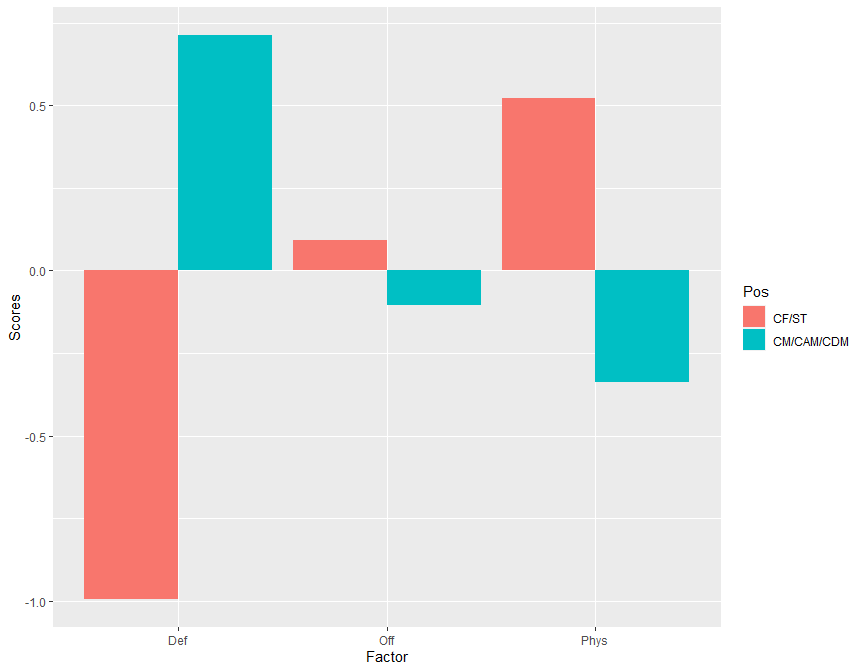
\includegraphics{Kutis_Skuska_markdown_files/figure-latex/unnamed-chunk-15-1.pdf}

In the next step we will apply LDA on FA tranformed dataset.

\begin{Shaded}
\begin{Highlighting}[]
\CommentTok{\# Useful libs}
\FunctionTok{library}\NormalTok{(caret)}
\end{Highlighting}
\end{Shaded}

\begin{verbatim}
## Loading required package: lattice
\end{verbatim}

\begin{verbatim}
## 
## Attaching package: 'caret'
\end{verbatim}

\begin{verbatim}
## The following object is masked from 'package:purrr':
## 
##     lift
\end{verbatim}

\begin{Shaded}
\begin{Highlighting}[]
\FunctionTok{library}\NormalTok{(ROCR)}
\end{Highlighting}
\end{Shaded}

\begin{verbatim}
## Warning: package 'ROCR' was built under R version 4.1.2
\end{verbatim}

Look to see whether data are normally distributed. It could look more
normal, but it isn't bad either. The reason for the distribution in Def
is that we have midfielders who are similar in this aspect to the
attackers (score really low in defense). Than there are
midfielders/attackers like Roberto Firmino, who have great defending as
they're useful for quickly regaining control high up the pitch after
loosing posession.

\begin{Shaded}
\begin{Highlighting}[]
\CommentTok{\# Data vyzeraju aproximativne normalne}
\NormalTok{fifa.fa }\SpecialCharTok{\%\textgreater{}\%}
\NormalTok{    dplyr}\SpecialCharTok{::}\FunctionTok{select}\NormalTok{(}\SpecialCharTok{{-}}\NormalTok{Name) }\SpecialCharTok{\%\textgreater{}\%}
    \FunctionTok{pivot\_longer}\NormalTok{(}\SpecialCharTok{{-}}\NormalTok{Pos, }\AttributeTok{names\_to =} \StringTok{"Variable"}\NormalTok{, }\AttributeTok{values\_to =} \StringTok{"Value"}\NormalTok{) }\SpecialCharTok{\%\textgreater{}\%}
    \FunctionTok{ggplot}\NormalTok{(}\FunctionTok{aes}\NormalTok{(}\AttributeTok{x =}\NormalTok{ Value, }\AttributeTok{y =}\NormalTok{ ..density.., }\AttributeTok{color =}\NormalTok{ Variable)) }\SpecialCharTok{+}
    \FunctionTok{geom\_histogram}\NormalTok{(}\AttributeTok{position =} \StringTok{"identity"}\NormalTok{,}
                   \AttributeTok{fill =} \StringTok{"azure2"}\NormalTok{,}
                   \AttributeTok{alpha =} \DecValTok{1}\NormalTok{) }\SpecialCharTok{+}
    \FunctionTok{geom\_density}\NormalTok{(}\AttributeTok{alpha =} \DecValTok{1}\NormalTok{, ) }\SpecialCharTok{+}
    \FunctionTok{facet\_grid}\NormalTok{(Variable }\SpecialCharTok{\textasciitilde{}}\NormalTok{ .) }\SpecialCharTok{+}
    \FunctionTok{scale\_color\_brewer}\NormalTok{(}\AttributeTok{palette =} \StringTok{"Spectral"}\NormalTok{)}
\end{Highlighting}
\end{Shaded}

\begin{verbatim}
## `stat_bin()` using `bins = 30`. Pick better value with `binwidth`.
\end{verbatim}

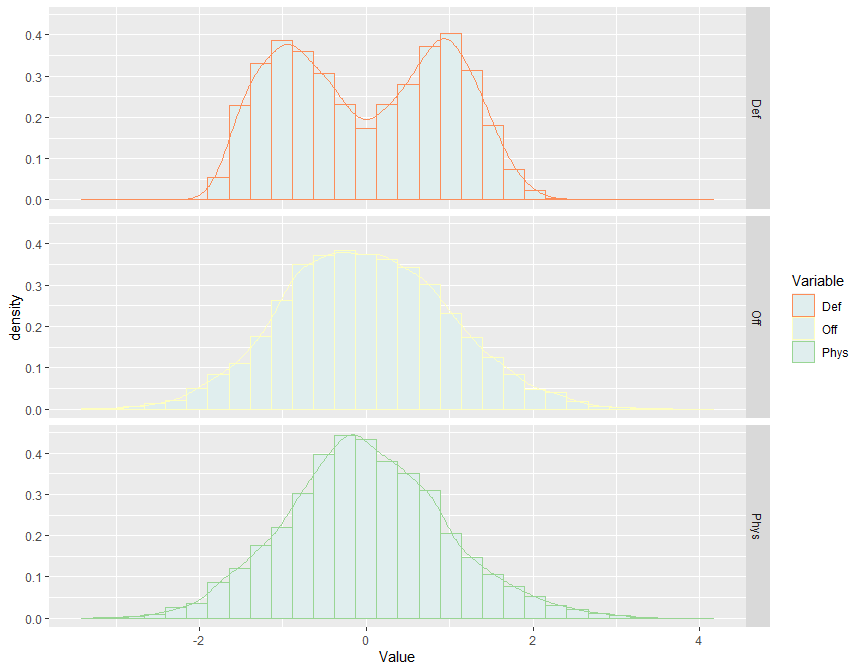
\includegraphics{Kutis_Skuska_markdown_files/figure-latex/unnamed-chunk-17-1.pdf}

\begin{Shaded}
\begin{Highlighting}[]
\CommentTok{\# Vyhodenie premennej meno pre LDA}
\NormalTok{fifa.fa }\OtherTok{\textless{}{-}}
\NormalTok{    fifa.fa }\SpecialCharTok{\%\textgreater{}\%}\NormalTok{ dplyr}\SpecialCharTok{::}\FunctionTok{select}\NormalTok{(}\SpecialCharTok{{-}}\NormalTok{Name) }\SpecialCharTok{\%\textgreater{}\%} \FunctionTok{mutate}\NormalTok{(}\AttributeTok{Pos =} \FunctionTok{factor}\NormalTok{(Pos, }\AttributeTok{levels =}
                                                                 \FunctionTok{c}\NormalTok{(}\StringTok{"CF/ST"}\NormalTok{, }\StringTok{"CM/CAM/CDM"}\NormalTok{)))}
\end{Highlighting}
\end{Shaded}

LDA on FA transformed data.

\begin{Shaded}
\begin{Highlighting}[]
\CommentTok{\# Train{-}Test split}
\NormalTok{train.index.fa }\OtherTok{\textless{}{-}}
\NormalTok{    fifa.fa}\SpecialCharTok{$}\NormalTok{Pos }\SpecialCharTok{\%\textgreater{}\%} \FunctionTok{createDataPartition}\NormalTok{(}\AttributeTok{p =} \FloatTok{0.75}\NormalTok{, }\AttributeTok{list =} \ConstantTok{FALSE}\NormalTok{)}
\NormalTok{train.data.fa }\OtherTok{\textless{}{-}}\NormalTok{ fifa.fa[train.index.fa,]}
\NormalTok{test.data.fa }\OtherTok{\textless{}{-}}\NormalTok{ fifa.fa[}\SpecialCharTok{{-}}\NormalTok{train.index.fa,]}

\CommentTok{\# Fitni model}
\NormalTok{model.fa }\OtherTok{\textless{}{-}} \FunctionTok{lda}\NormalTok{(Pos }\SpecialCharTok{\textasciitilde{}}\NormalTok{ ., }\AttributeTok{data =}\NormalTok{ train.data.fa,)}

\CommentTok{\# Predikcie}
\NormalTok{predictions.fa }\OtherTok{\textless{}{-}}\NormalTok{ model.fa }\SpecialCharTok{\%\textgreater{}\%} \FunctionTok{predict}\NormalTok{(test.data.fa)}

\DocumentationTok{\#\# Evaluation}
\CommentTok{\# Mozeme vidiet, ze model je pomerne dobry v tom ako predikuje hodnoty!}
\NormalTok{predictions.posteriors.fa }\OtherTok{\textless{}{-}}
    \FunctionTok{as.data.frame}\NormalTok{(predictions.fa}\SpecialCharTok{$}\NormalTok{posterior[, }\DecValTok{2}\NormalTok{])}
\NormalTok{pred.fa }\OtherTok{\textless{}{-}}
    \FunctionTok{prediction}\NormalTok{(predictions.posteriors.fa, test.data.fa}\SpecialCharTok{$}\NormalTok{Pos)}
\NormalTok{roc.perform.fa }\OtherTok{\textless{}{-}}
    \FunctionTok{performance}\NormalTok{(pred.fa, }\AttributeTok{measure =} \StringTok{"tpr"}\NormalTok{, }\AttributeTok{x.measure =} \StringTok{"fpr"}\NormalTok{)}
\NormalTok{auc.train.fa }\OtherTok{\textless{}{-}} \FunctionTok{performance}\NormalTok{(pred.fa, }\AttributeTok{measure =} \StringTok{"auc"}\NormalTok{)}
\NormalTok{auc.train.fa.val }\OtherTok{\textless{}{-}}\NormalTok{ auc.train.fa}\SpecialCharTok{@}\NormalTok{y.values}

\NormalTok{AUC\_FA }\OtherTok{\textless{}{-}} \FunctionTok{as.double}\NormalTok{(auc.train.fa.val)}
\end{Highlighting}
\end{Shaded}

ROC curve for FA - LDA

\begin{Shaded}
\begin{Highlighting}[]
\FunctionTok{plot}\NormalTok{(roc.perform.fa)}
\FunctionTok{title}\NormalTok{(}\StringTok{"ROC curve for FA transformed LDA predicton"}\NormalTok{)}
\FunctionTok{abline}\NormalTok{(}\AttributeTok{a =} \DecValTok{0}\NormalTok{, }\AttributeTok{b =} \DecValTok{1}\NormalTok{)}
\FunctionTok{grid}\NormalTok{()}
\FunctionTok{text}\NormalTok{(}\AttributeTok{x =}\NormalTok{ .}\DecValTok{25}\NormalTok{, }\AttributeTok{y =}\NormalTok{ .}\DecValTok{65}\NormalTok{ , }\FunctionTok{str\_glue}\NormalTok{(}\StringTok{"AUC = \{round(as.double(AUC\_FA), 3)\}"}\NormalTok{))}
\end{Highlighting}
\end{Shaded}

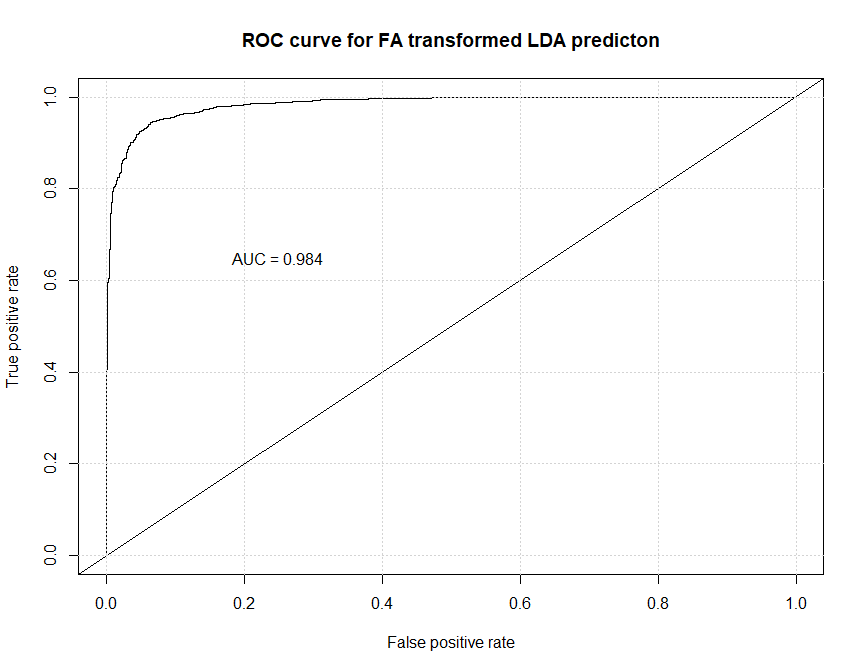
\includegraphics{Kutis_Skuska_markdown_files/figure-latex/unnamed-chunk-20-1.pdf}
LDA on raw data

\begin{Shaded}
\begin{Highlighting}[]
\CommentTok{\# Data}
\NormalTok{fifa.raw }\OtherTok{\textless{}{-}}
    \FunctionTok{cbind}\NormalTok{(}
\NormalTok{        data }\SpecialCharTok{\%\textgreater{}\%}
            \FunctionTok{filter}\NormalTok{(BestPos }\SpecialCharTok{\%in\%} \FunctionTok{c}\NormalTok{(}\StringTok{"CM/CAM/CDM"}\NormalTok{, }\StringTok{"CF/ST"}\NormalTok{)) }\SpecialCharTok{\%\textgreater{}\%}
            \FunctionTok{mutate}\NormalTok{(}\AttributeTok{BestPos =} \FunctionTok{factor}\NormalTok{(BestPos, }\AttributeTok{levels =} \FunctionTok{c}\NormalTok{(}
                \StringTok{"CM/CAM/CDM"}\NormalTok{, }\StringTok{"CF/ST"}
\NormalTok{            )))}
        \SpecialCharTok{\%\textgreater{}\%} \FunctionTok{na.omit}\NormalTok{() }\SpecialCharTok{\%\textgreater{}\%}\NormalTok{ dplyr}\SpecialCharTok{::}\FunctionTok{select}\NormalTok{(BestPos),}
\NormalTok{        fifa}
\NormalTok{    )}
\CommentTok{\# Preprocessing}
\NormalTok{preproces.param.raw }\OtherTok{\textless{}{-}}
\NormalTok{    fifa.raw }\SpecialCharTok{\%\textgreater{}\%} \FunctionTok{preProcess}\NormalTok{(}\AttributeTok{method =} \FunctionTok{c}\NormalTok{(}\StringTok{"center"}\NormalTok{, }\StringTok{"scale"}\NormalTok{))}
\NormalTok{fifa.raw.trans }\OtherTok{\textless{}{-}}\NormalTok{ preproces.param.raw }\SpecialCharTok{\%\textgreater{}\%} \FunctionTok{predict}\NormalTok{(fifa.raw)}

\CommentTok{\# Train{-}test split}
\NormalTok{train.index.raw }\OtherTok{\textless{}{-}}
\NormalTok{    fifa.raw}\SpecialCharTok{$}\NormalTok{BestPos }\SpecialCharTok{\%\textgreater{}\%} \FunctionTok{createDataPartition}\NormalTok{(}\AttributeTok{p =} \FloatTok{0.75}\NormalTok{, }\AttributeTok{list =} \ConstantTok{FALSE}\NormalTok{)}
\NormalTok{train.data.raw }\OtherTok{\textless{}{-}}\NormalTok{ fifa.raw.trans[train.index.raw,]}
\NormalTok{test.data.raw }\OtherTok{\textless{}{-}}\NormalTok{ fifa.raw.trans[}\SpecialCharTok{{-}}\NormalTok{train.index.raw,]}

\CommentTok{\# Fit the model}
\NormalTok{model.raw }\OtherTok{\textless{}{-}} \FunctionTok{lda}\NormalTok{(BestPos }\SpecialCharTok{\textasciitilde{}}\NormalTok{ ., }\AttributeTok{data =}\NormalTok{ train.data.raw)}

\CommentTok{\# Predikcie}
\NormalTok{predictions.raw }\OtherTok{\textless{}{-}}\NormalTok{ model.raw }\SpecialCharTok{\%\textgreater{}\%} \FunctionTok{predict}\NormalTok{(test.data.raw)}

\CommentTok{\# Evaluation}
\NormalTok{predictions.posteriors.raw }\OtherTok{\textless{}{-}}
    \FunctionTok{as.data.frame}\NormalTok{(predictions.raw}\SpecialCharTok{$}\NormalTok{posterior[, }\DecValTok{1}\NormalTok{])}

\NormalTok{pred.raw }\OtherTok{\textless{}{-}}
    \FunctionTok{prediction}\NormalTok{(predictions.posteriors.raw, test.data.raw}\SpecialCharTok{$}\NormalTok{BestPos)}
\NormalTok{roc.perform.raw }\OtherTok{\textless{}{-}}
    \FunctionTok{performance}\NormalTok{(pred.raw, }\AttributeTok{measure =} \StringTok{"tpr"}\NormalTok{, }\AttributeTok{x.measure =} \StringTok{"fpr"}\NormalTok{)}
\NormalTok{auc.train.raw }\OtherTok{\textless{}{-}} \FunctionTok{performance}\NormalTok{(pred.raw, }\AttributeTok{measure =} \StringTok{"auc"}\NormalTok{)}
\NormalTok{auc.train.raw.val }\OtherTok{\textless{}{-}}\NormalTok{ auc.train.raw}\SpecialCharTok{@}\NormalTok{y.values}
\NormalTok{AUC\_RAW }\OtherTok{\textless{}{-}} \FunctionTok{as.double}\NormalTok{(auc.train.raw.val)}
\end{Highlighting}
\end{Shaded}

ROC Curve for raw data LDA

\begin{Shaded}
\begin{Highlighting}[]
\FunctionTok{plot}\NormalTok{(roc.perform.raw)}
\FunctionTok{abline}\NormalTok{(}\AttributeTok{a =} \DecValTok{0}\NormalTok{, }\AttributeTok{b =} \DecValTok{1}\NormalTok{)}
\FunctionTok{title}\NormalTok{(}\StringTok{"ROC Curve for non{-}transformed variables LDA prediction"}\NormalTok{)}
\FunctionTok{grid}\NormalTok{()}
\FunctionTok{text}\NormalTok{(}\AttributeTok{x =}\NormalTok{ .}\DecValTok{25}\NormalTok{, }\AttributeTok{y =}\NormalTok{ .}\DecValTok{65}\NormalTok{ , }\FunctionTok{paste}\NormalTok{(}\StringTok{"AUC = "}\NormalTok{, }\FunctionTok{round}\NormalTok{(AUC\_RAW, }\DecValTok{3}\NormalTok{), }\AttributeTok{sep =} \StringTok{""}\NormalTok{))}
\end{Highlighting}
\end{Shaded}

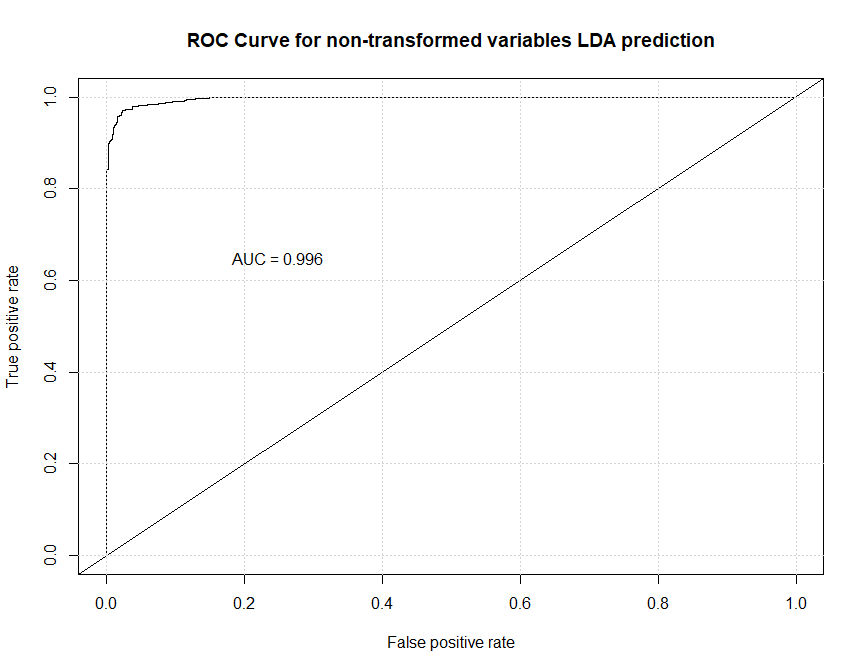
\includegraphics{Kutis_Skuska_markdown_files/figure-latex/unnamed-chunk-22-1.pdf}
Visualization of model on new LDA transformed axis

\begin{Shaded}
\begin{Highlighting}[]
\CommentTok{\# Prepare data for visualization}
\NormalTok{lda.raw.viz }\OtherTok{\textless{}{-}}
    \FunctionTok{as.data.frame}\NormalTok{(}\FunctionTok{cbind}\NormalTok{(}
        \FunctionTok{as.character}\NormalTok{(test.data.raw}\SpecialCharTok{$}\NormalTok{BestPos),}
\NormalTok{        predictions.raw}\SpecialCharTok{$}\NormalTok{x,}
        \FunctionTok{as.character}\NormalTok{(predictions.raw}\SpecialCharTok{$}\NormalTok{class)}
\NormalTok{    ))}

\FunctionTok{colnames}\NormalTok{(lda.raw.viz) }\OtherTok{\textless{}{-}} \FunctionTok{c}\NormalTok{(}\StringTok{"Act\_class"}\NormalTok{, }\StringTok{"LD1"}\NormalTok{, }\StringTok{"Pred\_class"}\NormalTok{)}

\NormalTok{lda.raw.viz }\OtherTok{\textless{}{-}}\NormalTok{ lda.raw.viz }\SpecialCharTok{\%\textgreater{}\%}
    \FunctionTok{as\_tibble}\NormalTok{() }\SpecialCharTok{\%\textgreater{}\%}
    \FunctionTok{mutate}\NormalTok{(}\AttributeTok{Pred\_OK =} \FunctionTok{as.factor}\NormalTok{(}
        \FunctionTok{case\_when}\NormalTok{(Act\_class }\SpecialCharTok{==}\NormalTok{ Pred\_class }\SpecialCharTok{\textasciitilde{}} \ConstantTok{TRUE}\NormalTok{,}
\NormalTok{                  Act\_class }\SpecialCharTok{!=}\NormalTok{ Pred\_class }\SpecialCharTok{\textasciitilde{}} \ConstantTok{FALSE}\NormalTok{)}
\NormalTok{    ))}
\NormalTok{lda.raw.viz}
\end{Highlighting}
\end{Shaded}

\begin{verbatim}
## # A tibble: 1,769 x 4
##    Act_class  LD1               Pred_class Pred_OK
##    <chr>      <chr>             <chr>      <fct>  
##  1 CM/CAM/CDM -1.12073079784837 CM/CAM/CDM TRUE   
##  2 CM/CAM/CDM 0.352330185805261 CM/CAM/CDM TRUE   
##  3 CM/CAM/CDM -1.27729239278172 CM/CAM/CDM TRUE   
##  4 CM/CAM/CDM -1.42295166862054 CM/CAM/CDM TRUE   
##  5 CM/CAM/CDM -1.46973510281046 CM/CAM/CDM TRUE   
##  6 CF/ST      3.2451983156624   CF/ST      TRUE   
##  7 CF/ST      2.2477996041084   CF/ST      TRUE   
##  8 CM/CAM/CDM -1.62904917984021 CM/CAM/CDM TRUE   
##  9 CM/CAM/CDM -1.11763803734919 CM/CAM/CDM TRUE   
## 10 CM/CAM/CDM -0.7900459968233  CM/CAM/CDM TRUE   
## # ... with 1,759 more rows
\end{verbatim}

\begin{Shaded}
\begin{Highlighting}[]
\CommentTok{\# Resulting visualization}
\FunctionTok{library}\NormalTok{(ggthemes)   }\CommentTok{\# Themes library}
\end{Highlighting}
\end{Shaded}

\begin{verbatim}
## Warning: package 'ggthemes' was built under R version 4.1.2
\end{verbatim}

\begin{Shaded}
\begin{Highlighting}[]
\NormalTok{lda.raw.viz }\SpecialCharTok{\%\textgreater{}\%}
    \FunctionTok{ggplot}\NormalTok{(}\FunctionTok{aes}\NormalTok{(}\AttributeTok{x =}\NormalTok{ LD1, }\AttributeTok{y =} \FunctionTok{rep}\NormalTok{(}\DecValTok{0}\NormalTok{, }\FunctionTok{length}\NormalTok{(LD1)))) }\SpecialCharTok{+}
    \FunctionTok{geom\_jitter}\NormalTok{(}\FunctionTok{aes}\NormalTok{(}\AttributeTok{color =}\NormalTok{ Act\_class)) }\SpecialCharTok{+}
    \FunctionTok{geom\_jitter}\NormalTok{(}
        \AttributeTok{data =}\NormalTok{ lda.raw.viz }\SpecialCharTok{\%\textgreater{}\%}
            \FunctionTok{filter}\NormalTok{(Pred\_OK }\SpecialCharTok{==} \ConstantTok{FALSE}\NormalTok{),}
        \AttributeTok{pch =} \DecValTok{21}\NormalTok{,}
        \AttributeTok{size =} \DecValTok{3}\NormalTok{,}
        \AttributeTok{color =} \StringTok{"red"}\NormalTok{,}
        \AttributeTok{fill =} \StringTok{"red"}\NormalTok{,}
        \AttributeTok{alpha =} \FloatTok{0.5}
\NormalTok{    ) }\SpecialCharTok{+}
    \FunctionTok{scale\_color\_manual}\NormalTok{(}\AttributeTok{name=} \StringTok{"Skutočné hodnoty"}\NormalTok{,}
                       \AttributeTok{values =} \FunctionTok{c}\NormalTok{(}\StringTok{"CM/ST"} \OtherTok{=} \StringTok{"darkgrey"}\NormalTok{, }\StringTok{"CM/CAM/CDM"} \OtherTok{=} \StringTok{"blue"}\NormalTok{),}
\NormalTok{                       ) }\SpecialCharTok{+}
    \FunctionTok{theme\_economist}\NormalTok{() }\SpecialCharTok{+} 
    \FunctionTok{labs}\NormalTok{(}\AttributeTok{y =} \StringTok{"Jittered 1D"}\NormalTok{,}
         \AttributeTok{title =} \StringTok{"Positions of observations on LDA transformed axis"}
\NormalTok{    ) }\SpecialCharTok{+} 
    \FunctionTok{theme}\NormalTok{(}
        \CommentTok{\# Parametre osi}
        \AttributeTok{axis.ticks.y =} \FunctionTok{element\_blank}\NormalTok{(),}
        \AttributeTok{axis.line =} \FunctionTok{element\_line}\NormalTok{(}\AttributeTok{color=}\StringTok{"black"}\NormalTok{),}
        \AttributeTok{axis.text =} \FunctionTok{element\_blank}\NormalTok{(),}
        \CommentTok{\# Grid prec}
        \AttributeTok{panel.grid.major =} \FunctionTok{element\_blank}\NormalTok{(),}
        \AttributeTok{panel.grid.minor =} \FunctionTok{element\_blank}\NormalTok{(),}
        \AttributeTok{legend.title =} \FunctionTok{element\_text}\NormalTok{(}\AttributeTok{size=}\DecValTok{15}\NormalTok{)}
\NormalTok{    ) }\SpecialCharTok{+}
    \CommentTok{\# Zvacsi velkosti v legende}
    \FunctionTok{guides}\NormalTok{(}
        \AttributeTok{colour =} \FunctionTok{guide\_legend}\NormalTok{(}\AttributeTok{override.aes =} \FunctionTok{list}\NormalTok{(}\AttributeTok{size=}\DecValTok{7}\NormalTok{))}
\NormalTok{        )}
\end{Highlighting}
\end{Shaded}

\includegraphics{Kutis_Skuska_markdown_files/figure-latex/unnamed-chunk-23-1.pdf}
Confusion Matrix

\begin{Shaded}
\begin{Highlighting}[]
\NormalTok{confusion.mx }\OtherTok{\textless{}{-}} \FunctionTok{confusionMatrix}\NormalTok{(}
    \AttributeTok{data =} \FunctionTok{as.factor}\NormalTok{(lda.raw.viz}\SpecialCharTok{$}\NormalTok{Pred\_class),}
    \AttributeTok{reference =} \FunctionTok{as.factor}\NormalTok{(lda.raw.viz}\SpecialCharTok{$}\NormalTok{Act\_class),}
    \AttributeTok{dnn =} \FunctionTok{c}\NormalTok{(}\StringTok{"Prediction"}\NormalTok{, }\StringTok{"Reference"}\NormalTok{),}
\NormalTok{)}
\NormalTok{confusion.mx}
\end{Highlighting}
\end{Shaded}

\begin{verbatim}
## Confusion Matrix and Statistics
## 
##             Reference
## Prediction   CF/ST CM/CAM/CDM
##   CF/ST        632         39
##   CM/CAM/CDM    20       1078
##                                           
##                Accuracy : 0.9666          
##                  95% CI : (0.9572, 0.9745)
##     No Information Rate : 0.6314          
##     P-Value [Acc > NIR] : < 2e-16         
##                                           
##                   Kappa : 0.9288          
##                                           
##  Mcnemar's Test P-Value : 0.01911         
##                                           
##             Sensitivity : 0.9693          
##             Specificity : 0.9651          
##          Pos Pred Value : 0.9419          
##          Neg Pred Value : 0.9818          
##              Prevalence : 0.3686          
##          Detection Rate : 0.3573          
##    Detection Prevalence : 0.3793          
##       Balanced Accuracy : 0.9672          
##                                           
##        'Positive' Class : CF/ST           
## 
\end{verbatim}

To this point, we produced two LDA classifications. One for FA
transformed data and one for not transformed data. From results it seems
that the latter performs better. But still, we should verify wheter it
does. We will create 100 runs of both classifications, get AUC and
compare these two with t-test.

FA transformed LDA classification - 1000 runs

\begin{Shaded}
\begin{Highlighting}[]
\CommentTok{\# seed}
\FunctionTok{set.seed}\NormalTok{(}\DecValTok{123}\NormalTok{)}

\NormalTok{AUC\_FA }\OtherTok{\textless{}{-}} \FunctionTok{rep}\NormalTok{(}\DecValTok{0}\NormalTok{, }\DecValTok{1000}\NormalTok{) }\CommentTok{\# Empty vector for storing results of classification.}
\ControlFlowTok{for}\NormalTok{ (i }\ControlFlowTok{in} \DecValTok{1}\SpecialCharTok{:}\DecValTok{1000}\NormalTok{) \{}
    \CommentTok{\# Train{-}Test split}
\NormalTok{    train.index.fa }\OtherTok{\textless{}{-}}
\NormalTok{        fifa.fa}\SpecialCharTok{$}\NormalTok{Pos }\SpecialCharTok{\%\textgreater{}\%} \FunctionTok{createDataPartition}\NormalTok{(}\AttributeTok{p =} \FloatTok{0.75}\NormalTok{, }\AttributeTok{list =} \ConstantTok{FALSE}\NormalTok{)}
\NormalTok{    train.data.fa }\OtherTok{\textless{}{-}}\NormalTok{ fifa.fa[train.index.fa,]}
\NormalTok{    test.data.fa }\OtherTok{\textless{}{-}}\NormalTok{ fifa.fa[}\SpecialCharTok{{-}}\NormalTok{train.index.fa,]}
    
    \CommentTok{\# Fit the model}
\NormalTok{    model.fa }\OtherTok{\textless{}{-}} \FunctionTok{lda}\NormalTok{(Pos }\SpecialCharTok{\textasciitilde{}}\NormalTok{ ., }\AttributeTok{data =}\NormalTok{ train.data.fa,)}
    
    \CommentTok{\# Predikcie}
\NormalTok{    predictions.fa }\OtherTok{\textless{}{-}}\NormalTok{ model.fa }\SpecialCharTok{\%\textgreater{}\%} \FunctionTok{predict}\NormalTok{(test.data.fa)}
    
    \CommentTok{\# Evaluation}
\NormalTok{    predictions.posteriors.fa }\OtherTok{\textless{}{-}}
        \FunctionTok{as.data.frame}\NormalTok{(predictions.fa}\SpecialCharTok{$}\NormalTok{posterior[, }\DecValTok{2}\NormalTok{])}

\NormalTok{    pred.fa }\OtherTok{\textless{}{-}}
        \FunctionTok{prediction}\NormalTok{(predictions.posteriors.fa, test.data.fa}\SpecialCharTok{$}\NormalTok{Pos)}
\NormalTok{    roc.perform.fa }\OtherTok{\textless{}{-}}
        \FunctionTok{performance}\NormalTok{(pred.fa, }\AttributeTok{measure =} \StringTok{"tpr"}\NormalTok{, }\AttributeTok{x.measure =} \StringTok{"fpr"}\NormalTok{)}
\NormalTok{    auc.train.fa }\OtherTok{\textless{}{-}} \FunctionTok{performance}\NormalTok{(pred.fa, }\AttributeTok{measure =} \StringTok{"auc"}\NormalTok{)}
\NormalTok{    auc.train.fa.val }\OtherTok{\textless{}{-}}\NormalTok{ auc.train.fa}\SpecialCharTok{@}\NormalTok{y.values}
    
    \CommentTok{\# Save the results to vector of AUC values for FA transformed LDA}
\NormalTok{    AUC\_FA[i] }\OtherTok{\textless{}{-}} \FunctionTok{as.double}\NormalTok{(auc.train.fa.val)}
\NormalTok{\}}
\end{Highlighting}
\end{Shaded}

Non-transformed LDA classification - 1000 runs (it can take longer as
there are more columns)

\begin{Shaded}
\begin{Highlighting}[]
\NormalTok{AUC\_RAW }\OtherTok{\textless{}{-}} \FunctionTok{rep}\NormalTok{(}\DecValTok{0}\NormalTok{, }\DecValTok{1000}\NormalTok{) }\CommentTok{\# Empty vector for storing results of classification.}
\ControlFlowTok{for}\NormalTok{ (i }\ControlFlowTok{in} \DecValTok{1}\SpecialCharTok{:}\DecValTok{1000}\NormalTok{) \{}
    \CommentTok{\# Preprocessing}
\NormalTok{    preproces.param.raw }\OtherTok{\textless{}{-}}
\NormalTok{        fifa.raw }\SpecialCharTok{\%\textgreater{}\%} \FunctionTok{preProcess}\NormalTok{(}\AttributeTok{method =} \FunctionTok{c}\NormalTok{(}\StringTok{"center"}\NormalTok{, }\StringTok{"scale"}\NormalTok{))}
\NormalTok{    fifa.raw.trans }\OtherTok{\textless{}{-}}\NormalTok{ preproces.param.raw }\SpecialCharTok{\%\textgreater{}\%} \FunctionTok{predict}\NormalTok{(fifa.raw)}
    
    \CommentTok{\# Train{-}test split}
\NormalTok{    train.index.raw }\OtherTok{\textless{}{-}}
\NormalTok{        fifa.raw}\SpecialCharTok{$}\NormalTok{BestPos }\SpecialCharTok{\%\textgreater{}\%} \FunctionTok{createDataPartition}\NormalTok{(}\AttributeTok{p =} \FloatTok{0.75}\NormalTok{, }\AttributeTok{list =} \ConstantTok{FALSE}\NormalTok{)}
\NormalTok{    train.data.raw }\OtherTok{\textless{}{-}}\NormalTok{ fifa.raw.trans[train.index.raw, ]}
\NormalTok{    test.data.raw }\OtherTok{\textless{}{-}}\NormalTok{ fifa.raw.trans[}\SpecialCharTok{{-}}\NormalTok{train.index.raw, ]}

    \CommentTok{\# Fit the model}
\NormalTok{    model.raw }\OtherTok{\textless{}{-}} \FunctionTok{lda}\NormalTok{(BestPos }\SpecialCharTok{\textasciitilde{}}\NormalTok{ ., }\AttributeTok{data =}\NormalTok{ fifa.raw.trans)}

    \CommentTok{\# Predictions}
\NormalTok{    predictions.raw }\OtherTok{\textless{}{-}}\NormalTok{ model.raw }\SpecialCharTok{\%\textgreater{}\%} \FunctionTok{predict}\NormalTok{(test.data.raw)}

    \CommentTok{\# Evaluation}
\NormalTok{    predictions.posteriors.raw }\OtherTok{\textless{}{-}}
        \FunctionTok{as.data.frame}\NormalTok{(predictions.raw}\SpecialCharTok{$}\NormalTok{posterior[, }\DecValTok{1}\NormalTok{])}

\NormalTok{    pred.raw }\OtherTok{\textless{}{-}}
        \FunctionTok{prediction}\NormalTok{(predictions.posteriors.raw, test.data.raw}\SpecialCharTok{$}\NormalTok{BestPos)}
    
\NormalTok{    roc.perform.raw }\OtherTok{\textless{}{-}}
        \FunctionTok{performance}\NormalTok{(pred.raw, }\AttributeTok{measure =} \StringTok{"tpr"}\NormalTok{, }\AttributeTok{x.measure =} \StringTok{"fpr"}\NormalTok{)}
\NormalTok{    auc.train.raw }\OtherTok{\textless{}{-}} \FunctionTok{performance}\NormalTok{(pred.raw, }\AttributeTok{measure =} \StringTok{"auc"}\NormalTok{)}
\NormalTok{    auc.train.raw.val }\OtherTok{\textless{}{-}}\NormalTok{ auc.train.raw}\SpecialCharTok{@}\NormalTok{y.values}
    
    \CommentTok{\# Save the results to vector of AUC values }
\NormalTok{    AUC\_RAW[i] }\OtherTok{\textless{}{-}} \FunctionTok{as.double}\NormalTok{(auc.train.raw.val)}
\NormalTok{\}}
\end{Highlighting}
\end{Shaded}

Paired T-test: Two approaches classification

\begin{Shaded}
\begin{Highlighting}[]
\FunctionTok{library}\NormalTok{(BSDA)}
\end{Highlighting}
\end{Shaded}

\begin{verbatim}
## Warning: package 'BSDA' was built under R version 4.1.2
\end{verbatim}

\begin{verbatim}
## 
## Attaching package: 'BSDA'
\end{verbatim}

\begin{verbatim}
## The following object is masked from 'package:datasets':
## 
##     Orange
\end{verbatim}

\begin{Shaded}
\begin{Highlighting}[]
\FunctionTok{t.test}\NormalTok{(}\AttributeTok{x=}\FunctionTok{as.double}\NormalTok{(AUC\_FA),}\AttributeTok{y=} \FunctionTok{as.double}\NormalTok{(AUC\_RAW), }\AttributeTok{paired=}\ConstantTok{TRUE}\NormalTok{, }\AttributeTok{alternative=}\StringTok{"less"}\NormalTok{)}
\end{Highlighting}
\end{Shaded}

\begin{verbatim}
## 
##  Paired t-test
## 
## data:  as.double(AUC_FA) and as.double(AUC_RAW)
## t = -164.49, df = 999, p-value < 2.2e-16
## alternative hypothesis: true difference in means is less than 0
## 95 percent confidence interval:
##         -Inf -0.01081214
## sample estimates:
## mean of the differences 
##             -0.01092145
\end{verbatim}

\begin{Shaded}
\begin{Highlighting}[]
\FunctionTok{print}\NormalTok{(}\StringTok{"Vysledok testu ukazuje, ze LDA model postaveny na nepretranformovanych datach je lepsi!"}\NormalTok{)}
\end{Highlighting}
\end{Shaded}

\begin{verbatim}
## [1] "Vysledok testu ukazuje, ze LDA model postaveny na nepretranformovanych datach je lepsi!"
\end{verbatim}

\end{document}
